\section{Hyperparameter optimization}

Now that the models have been defined in the previous section, an Hyperparameter (HP) optimization phase 
is needed.
The HP choice is essential to obtain the best performance of a neural network, and it can significantly influence the model's ability to generalize to unseen data. 
\noindent
Only 4 Hyperparameters [with related possible values] are considered in the models:
\begin{enumerate}
    \item Learning rate: the step size at each iteration while moving toward a minimum of the loss function; it controls how much the model weights are updated during training. $[0.0001,0.01]$
    \item Batch Size: the number of samples used to compute each update of the model weights; it influences the stability and speed of the training process. $\{16,32,64,128\}$
    \item Dropout percentage: the fraction of input units to drop during training to prevent overfitting; it helps improve the model's ability to generalize. $[0,0.5]$
    \item Momentum: coefficient that accelerates optimization by accumulating past gradients; helps achieve faster and more stable convergence. $[0,1]$
\end{enumerate}

Given the use of state-of-the-art architectures, other HPs such as activation functions, layers number, and layer types have not been changed.

\subsection{Search Algorithms for HPO}
The search for optimal HP values can be done, among others, in two ways: manually setting them based on prior experience or 
intuition, or using automated search algorithms.

Although manual testing remains one of the most widely used methods, especially in the student environment, it
requires a deep knowledge of the used algorithms and their HPs meaining. In addition, it has been found that 
a manual procedure is ineffective for several problems due to different factors, such as the high dimensionality 
of the hyperparameter space, the presence of complex interactions between hyperparameters, and the computational 
cost of exhaustively evaluating all possible combinations \cite{YANG2020295}. For this reason, manual testing
was discarded in favor of using a search algorithm.

\noindent
More formally, a HPs optimization problem aims to find the HPs configuration $\bm{x}^* \in X$ such that:
$$ \bm{x}^* = \text{arg}\underset{\bm{x}\in X}{\min}f(\bm{x}) $$
where $X$ is the search space containing all the possible hyperparameter configurations, and $f$ is the
objective function (e.g., validation loss or error) to be minimized. A search algorithm is an heuristic algorithm
whose goal is to achieve the optimal, or near-optimal, HPs configuration within a given budget, which can be of
time or computational resources.

In the next section the simplest search algorithms will be shown. Given the low number of HPs, the use of more
sophisticated algorithms like Bayesan optimization or Gradient based optimization was not deemed necessary
in favor of a simpler random search.

\subsubsection{Grid search}
Grid search is the most straightforward hyperparameter tuning algorithm. It discretizes the search space of each
hyperparameter and evaluates all possible combinations. The combination that yields the best average performance 
is selected as the optimal set of hyperparameters.

It may happen that the well-performance regions cannot be detected, however, to identify the global optimums, the following procedure can be performed:
\begin{enumerate}
    \item Start with a large search space and step size;
    \item Narrow the search space and step size based on the best performance regions found on the previous step;
    \item Repeat step 2 multiple times until an optimum is reached.
\end{enumerate}

Grid search can be easily be implemented and parallelized but, being de facto brute force, it's ineffective with
a high number of HPs. In fact, its computational complexity is $O(n^k)$ where $k$ is the HPs number and $n$ is the
number of possible values.

\subsubsection{Random search}
Random search is a search algorithm similar to grid search. Instead of exploring all the values in the search 
space, random search randomly samples hyperparameter combinations from the defined ranges or sets. Each sampled 
configuration is evaluated, and the best-performing set is selected.

With a limited budget, random search is able to explore a larger search space than grid search by reducing the 
probability of wasting time on small poor-performance regions. Its computational complexity is $O(n)$, where $n$ 
is the number of sampled configurations defined before the optimization process starts.

\begin{figure}[H]
    \centering
    \begin{minipage}{0.45\textwidth}
        \resizebox{\textwidth}{!}{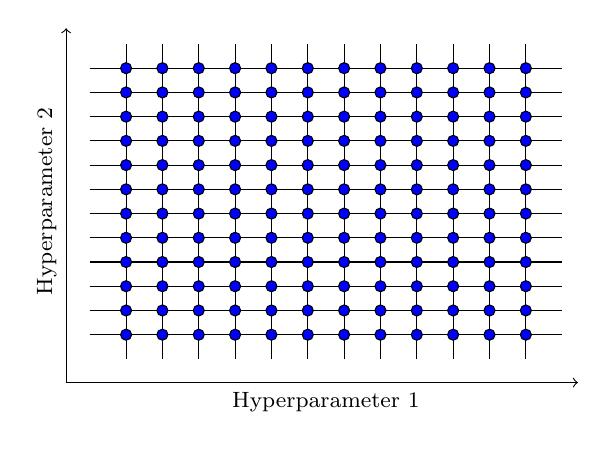
\begin{tikzpicture}
	%START
	\draw[->] (-0.3, -0.3) -- (6.2, -0.3);
	\draw[->] (-0.3, -0.3) -- (-0.3, 4.2);
	\draw (0.46153846153846156, 0.0) -- (0.46153846153846156, 4.0);
	\draw (0.9230769230769231, 0.0) -- (0.9230769230769231, 4.0);
	\draw (1.3846153846153846, 0.0) -- (1.3846153846153846, 4.0);
	\draw (1.8461538461538463, 0.0) -- (1.8461538461538463, 4.0);
	\draw (2.307692307692308, 0.0) -- (2.307692307692308, 4.0);
	\draw (2.769230769230769, 0.0) -- (2.769230769230769, 4.0);
	\draw (3.230769230769231, 0.0) -- (3.230769230769231, 4.0);
	\draw (3.6923076923076925, 0.0) -- (3.6923076923076925, 4.0);
	\draw (4.153846153846154, 0.0) -- (4.153846153846154, 4.0);
	\draw (4.615384615384616, 0.0) -- (4.615384615384616, 4.0);
	\draw (5.0769230769230775, 0.0) -- (5.0769230769230775, 4.0);
	\draw (5.538461538461538, 0.0) -- (5.538461538461538, 4.0);
	\draw (0.0, 0.3076923076923077) -- (6.0, 0.3076923076923077);
	\draw (0.0, 0.6153846153846154) -- (6.0, 0.6153846153846154);
	\draw (0.0, 0.9230769230769231) -- (6.0, 0.9230769230769231);
	\draw (0.0, 1.2307692307692308) -- (6.0, 1.2307692307692308);
	\draw (0.0, 1.5384615384615385) -- (6.0, 1.5384615384615385);
	\draw (0.0, 1.8461538461538463) -- (6.0, 1.8461538461538463);
	\draw (0.0, 2.153846153846154) -- (6.0, 2.153846153846154);
	\draw (0.0, 2.4615384615384617) -- (6.0, 2.4615384615384617);
	\draw (0.0, 2.769230769230769) -- (6.0, 2.769230769230769);
	\draw (0.0, 3.076923076923077) -- (6.0, 3.076923076923077);
	\draw (0.0, 3.384615384615385) -- (6.0, 3.384615384615385);
	\draw (0.0, 3.6923076923076925) -- (6.0, 3.6923076923076925);
	\draw[fill=blue] (0.46153846153846156, 0.3076923076923077) circle (0.07);
	\draw[fill=blue] (0.46153846153846156, 0.6153846153846154) circle (0.07);
	\draw[fill=blue] (0.46153846153846156, 0.9230769230769231) circle (0.07);
	\draw[fill=blue] (0.46153846153846156, 1.2307692307692308) circle (0.07);
	\draw[fill=blue] (0.46153846153846156, 1.5384615384615385) circle (0.07);
	\draw[fill=blue] (0.46153846153846156, 1.8461538461538463) circle (0.07);
	\draw[fill=blue] (0.46153846153846156, 2.153846153846154) circle (0.07);
	\draw[fill=blue] (0.46153846153846156, 2.4615384615384617) circle (0.07);
	\draw[fill=blue] (0.46153846153846156, 2.769230769230769) circle (0.07);
	\draw[fill=blue] (0.46153846153846156, 3.076923076923077) circle (0.07);
	\draw[fill=blue] (0.46153846153846156, 3.384615384615385) circle (0.07);
	\draw[fill=blue] (0.46153846153846156, 3.6923076923076925) circle (0.07);
	\draw[fill=blue] (0.9230769230769231, 0.3076923076923077) circle (0.07);
	\draw[fill=blue] (0.9230769230769231, 0.6153846153846154) circle (0.07);
	\draw[fill=blue] (0.9230769230769231, 0.9230769230769231) circle (0.07);
	\draw[fill=blue] (0.9230769230769231, 1.2307692307692308) circle (0.07);
	\draw[fill=blue] (0.9230769230769231, 1.5384615384615385) circle (0.07);
	\draw[fill=blue] (0.9230769230769231, 1.8461538461538463) circle (0.07);
	\draw[fill=blue] (0.9230769230769231, 2.153846153846154) circle (0.07);
	\draw[fill=blue] (0.9230769230769231, 2.4615384615384617) circle (0.07);
	\draw[fill=blue] (0.9230769230769231, 2.769230769230769) circle (0.07);
	\draw[fill=blue] (0.9230769230769231, 3.076923076923077) circle (0.07);
	\draw[fill=blue] (0.9230769230769231, 3.384615384615385) circle (0.07);
	\draw[fill=blue] (0.9230769230769231, 3.6923076923076925) circle (0.07);
	\draw[fill=blue] (1.3846153846153846, 0.3076923076923077) circle (0.07);
	\draw[fill=blue] (1.3846153846153846, 0.6153846153846154) circle (0.07);
	\draw[fill=blue] (1.3846153846153846, 0.9230769230769231) circle (0.07);
	\draw[fill=blue] (1.3846153846153846, 1.2307692307692308) circle (0.07);
	\draw[fill=blue] (1.3846153846153846, 1.5384615384615385) circle (0.07);
	\draw[fill=blue] (1.3846153846153846, 1.8461538461538463) circle (0.07);
	\draw[fill=blue] (1.3846153846153846, 2.153846153846154) circle (0.07);
	\draw[fill=blue] (1.3846153846153846, 2.4615384615384617) circle (0.07);
	\draw[fill=blue] (1.3846153846153846, 2.769230769230769) circle (0.07);
	\draw[fill=blue] (1.3846153846153846, 3.076923076923077) circle (0.07);
	\draw[fill=blue] (1.3846153846153846, 3.384615384615385) circle (0.07);
	\draw[fill=blue] (1.3846153846153846, 3.6923076923076925) circle (0.07);
	\draw[fill=blue] (1.8461538461538463, 0.3076923076923077) circle (0.07);
	\draw[fill=blue] (1.8461538461538463, 0.6153846153846154) circle (0.07);
	\draw[fill=blue] (1.8461538461538463, 0.9230769230769231) circle (0.07);
	\draw[fill=blue] (1.8461538461538463, 1.2307692307692308) circle (0.07);
	\draw[fill=blue] (1.8461538461538463, 1.5384615384615385) circle (0.07);
	\draw[fill=blue] (1.8461538461538463, 1.8461538461538463) circle (0.07);
	\draw[fill=blue] (1.8461538461538463, 2.153846153846154) circle (0.07);
	\draw[fill=blue] (1.8461538461538463, 2.4615384615384617) circle (0.07);
	\draw[fill=blue] (1.8461538461538463, 2.769230769230769) circle (0.07);
	\draw[fill=blue] (1.8461538461538463, 3.076923076923077) circle (0.07);
	\draw[fill=blue] (1.8461538461538463, 3.384615384615385) circle (0.07);
	\draw[fill=blue] (1.8461538461538463, 3.6923076923076925) circle (0.07);
	\draw[fill=blue] (2.307692307692308, 0.3076923076923077) circle (0.07);
	\draw[fill=blue] (2.307692307692308, 0.6153846153846154) circle (0.07);
	\draw[fill=blue] (2.307692307692308, 0.9230769230769231) circle (0.07);
	\draw[fill=blue] (2.307692307692308, 1.2307692307692308) circle (0.07);
	\draw[fill=blue] (2.307692307692308, 1.5384615384615385) circle (0.07);
	\draw[fill=blue] (2.307692307692308, 1.8461538461538463) circle (0.07);
	\draw[fill=blue] (2.307692307692308, 2.153846153846154) circle (0.07);
	\draw[fill=blue] (2.307692307692308, 2.4615384615384617) circle (0.07);
	\draw[fill=blue] (2.307692307692308, 2.769230769230769) circle (0.07);
	\draw[fill=blue] (2.307692307692308, 3.076923076923077) circle (0.07);
	\draw[fill=blue] (2.307692307692308, 3.384615384615385) circle (0.07);
	\draw[fill=blue] (2.307692307692308, 3.6923076923076925) circle (0.07);
	\draw[fill=blue] (2.769230769230769, 0.3076923076923077) circle (0.07);
	\draw[fill=blue] (2.769230769230769, 0.6153846153846154) circle (0.07);
	\draw[fill=blue] (2.769230769230769, 0.9230769230769231) circle (0.07);
	\draw[fill=blue] (2.769230769230769, 1.2307692307692308) circle (0.07);
	\draw[fill=blue] (2.769230769230769, 1.5384615384615385) circle (0.07);
	\draw[fill=blue] (2.769230769230769, 1.8461538461538463) circle (0.07);
	\draw[fill=blue] (2.769230769230769, 2.153846153846154) circle (0.07);
	\draw[fill=blue] (2.769230769230769, 2.4615384615384617) circle (0.07);
	\draw[fill=blue] (2.769230769230769, 2.769230769230769) circle (0.07);
	\draw[fill=blue] (2.769230769230769, 3.076923076923077) circle (0.07);
	\draw[fill=blue] (2.769230769230769, 3.384615384615385) circle (0.07);
	\draw[fill=blue] (2.769230769230769, 3.6923076923076925) circle (0.07);
	\draw[fill=blue] (3.230769230769231, 0.3076923076923077) circle (0.07);
	\draw[fill=blue] (3.230769230769231, 0.6153846153846154) circle (0.07);
	\draw[fill=blue] (3.230769230769231, 0.9230769230769231) circle (0.07);
	\draw[fill=blue] (3.230769230769231, 1.2307692307692308) circle (0.07);
	\draw[fill=blue] (3.230769230769231, 1.5384615384615385) circle (0.07);
	\draw[fill=blue] (3.230769230769231, 1.8461538461538463) circle (0.07);
	\draw[fill=blue] (3.230769230769231, 2.153846153846154) circle (0.07);
	\draw[fill=blue] (3.230769230769231, 2.4615384615384617) circle (0.07);
	\draw[fill=blue] (3.230769230769231, 2.769230769230769) circle (0.07);
	\draw[fill=blue] (3.230769230769231, 3.076923076923077) circle (0.07);
	\draw[fill=blue] (3.230769230769231, 3.384615384615385) circle (0.07);
	\draw[fill=blue] (3.230769230769231, 3.6923076923076925) circle (0.07);
	\draw[fill=blue] (3.6923076923076925, 0.3076923076923077) circle (0.07);
	\draw[fill=blue] (3.6923076923076925, 0.6153846153846154) circle (0.07);
	\draw[fill=blue] (3.6923076923076925, 0.9230769230769231) circle (0.07);
	\draw[fill=blue] (3.6923076923076925, 1.2307692307692308) circle (0.07);
	\draw[fill=blue] (3.6923076923076925, 1.5384615384615385) circle (0.07);
	\draw[fill=blue] (3.6923076923076925, 1.8461538461538463) circle (0.07);
	\draw[fill=blue] (3.6923076923076925, 2.153846153846154) circle (0.07);
	\draw[fill=blue] (3.6923076923076925, 2.4615384615384617) circle (0.07);
	\draw[fill=blue] (3.6923076923076925, 2.769230769230769) circle (0.07);
	\draw[fill=blue] (3.6923076923076925, 3.076923076923077) circle (0.07);
	\draw[fill=blue] (3.6923076923076925, 3.384615384615385) circle (0.07);
	\draw[fill=blue] (3.6923076923076925, 3.6923076923076925) circle (0.07);
	\draw[fill=blue] (4.153846153846154, 0.3076923076923077) circle (0.07);
	\draw[fill=blue] (4.153846153846154, 0.6153846153846154) circle (0.07);
	\draw[fill=blue] (4.153846153846154, 0.9230769230769231) circle (0.07);
	\draw[fill=blue] (4.153846153846154, 1.2307692307692308) circle (0.07);
	\draw[fill=blue] (4.153846153846154, 1.5384615384615385) circle (0.07);
	\draw[fill=blue] (4.153846153846154, 1.8461538461538463) circle (0.07);
	\draw[fill=blue] (4.153846153846154, 2.153846153846154) circle (0.07);
	\draw[fill=blue] (4.153846153846154, 2.4615384615384617) circle (0.07);
	\draw[fill=blue] (4.153846153846154, 2.769230769230769) circle (0.07);
	\draw[fill=blue] (4.153846153846154, 3.076923076923077) circle (0.07);
	\draw[fill=blue] (4.153846153846154, 3.384615384615385) circle (0.07);
	\draw[fill=blue] (4.153846153846154, 3.6923076923076925) circle (0.07);
	\draw[fill=blue] (4.615384615384616, 0.3076923076923077) circle (0.07);
	\draw[fill=blue] (4.615384615384616, 0.6153846153846154) circle (0.07);
	\draw[fill=blue] (4.615384615384616, 0.9230769230769231) circle (0.07);
	\draw[fill=blue] (4.615384615384616, 1.2307692307692308) circle (0.07);
	\draw[fill=blue] (4.615384615384616, 1.5384615384615385) circle (0.07);
	\draw[fill=blue] (4.615384615384616, 1.8461538461538463) circle (0.07);
	\draw[fill=blue] (4.615384615384616, 2.153846153846154) circle (0.07);
	\draw[fill=blue] (4.615384615384616, 2.4615384615384617) circle (0.07);
	\draw[fill=blue] (4.615384615384616, 2.769230769230769) circle (0.07);
	\draw[fill=blue] (4.615384615384616, 3.076923076923077) circle (0.07);
	\draw[fill=blue] (4.615384615384616, 3.384615384615385) circle (0.07);
	\draw[fill=blue] (4.615384615384616, 3.6923076923076925) circle (0.07);
	\draw[fill=blue] (5.0769230769230775, 0.3076923076923077) circle (0.07);
	\draw[fill=blue] (5.0769230769230775, 0.6153846153846154) circle (0.07);
	\draw[fill=blue] (5.0769230769230775, 0.9230769230769231) circle (0.07);
	\draw[fill=blue] (5.0769230769230775, 1.2307692307692308) circle (0.07);
	\draw[fill=blue] (5.0769230769230775, 1.5384615384615385) circle (0.07);
	\draw[fill=blue] (5.0769230769230775, 1.8461538461538463) circle (0.07);
	\draw[fill=blue] (5.0769230769230775, 2.153846153846154) circle (0.07);
	\draw[fill=blue] (5.0769230769230775, 2.4615384615384617) circle (0.07);
	\draw[fill=blue] (5.0769230769230775, 2.769230769230769) circle (0.07);
	\draw[fill=blue] (5.0769230769230775, 3.076923076923077) circle (0.07);
	\draw[fill=blue] (5.0769230769230775, 3.384615384615385) circle (0.07);
	\draw[fill=blue] (5.0769230769230775, 3.6923076923076925) circle (0.07);
	\draw[fill=blue] (5.538461538461538, 0.3076923076923077) circle (0.07);
	\draw[fill=blue] (5.538461538461538, 0.6153846153846154) circle (0.07);
	\draw[fill=blue] (5.538461538461538, 0.9230769230769231) circle (0.07);
	\draw[fill=blue] (5.538461538461538, 1.2307692307692308) circle (0.07);
	\draw[fill=blue] (5.538461538461538, 1.5384615384615385) circle (0.07);
	\draw[fill=blue] (5.538461538461538, 1.8461538461538463) circle (0.07);
	\draw[fill=blue] (5.538461538461538, 2.153846153846154) circle (0.07);
	\draw[fill=blue] (5.538461538461538, 2.4615384615384617) circle (0.07);
	\draw[fill=blue] (5.538461538461538, 2.769230769230769) circle (0.07);
	\draw[fill=blue] (5.538461538461538, 3.076923076923077) circle (0.07);
	\draw[fill=blue] (5.538461538461538, 3.384615384615385) circle (0.07);
	\draw[fill=blue] (5.538461538461538, 3.6923076923076925) circle (0.07);
	\node[below] at (3.0, -0.3) {\footnotesize Hyperparameter 1};
	\node[above,rotate=90] at (-0.3, 2.0) {\footnotesize Hyperparameter 2};
	%END
\end{tikzpicture}}
    \end{minipage}
    \begin{minipage}{0.45\textwidth}
        \resizebox{\textwidth}{!}{\input{tikz/randomSearch.tex}}
    \end{minipage}
    \vspace{-0.5em}
    \captionsetup{width=0.94\linewidth}
    \caption{Comparison between grid search(left) and random search(right) with 2 HPs\label{fig:grisSearch}}
\end{figure}

The random search and grid space problem is that every evaluation is independent of previous evaluations; 
thus, they waste massive time evaluating poorly-performance areas of the search space.

\subsection{Setup}
To perform the HPs optimization phase Ray Tune \cite{liaw2018tune}, an industrial standard tool for distributed HP 
tuning, was used. To find the optimal HPs configuration a random space was performed with the following search
spaces:
\begin{enumerate}
    \item Learning rate: the search was performed using \texttt{tune.loguniform} between $[0.0001,0.01]$, which 
    samples values $x$ such that $\log{x}$ is uniformly distributed between $\log{a}$ and $\log{b}$;
    \item Batch size: $\{16,32,64,128\}$;
    \item Dropout percentage: $[0,0.6]$ divided in 10 equally spaced points.
    \item Momentum: $[0,1]$ divided in 20 equally spaced points.
\end{enumerate}

\noindent
To run every HPs configuration trial an Asynchronous Successive Halving Algorithm (ASHA) scheduler
\cite{li2020massivelyparallelhyperparametertuning} was used. 

\subsubsection{Asynchronous Successive Halving Algorithm}
ASHA is an early stopping algorithm that efficiently 
allocates resources by quickly terminating underperforming trials and allocating more resources to promising ones.

More precisely, ASHA's procedure can be summarized as follows:
\begin{enumerate}
    \item Launch many trials, one per HPs configuration;
    \item Every trial is performed for at least $g$ time units;
    \item After $g$ time units all trials that have reached the same amount of time units are evaluated;
    \item Only a $1/r$ fraction of the best trials are kept, while the others are early stopped;
    \item The remaining trials continue to be performed and will be evaluated in the next round;
    \item Only the trials that survive all rounds are trained until the maximum number of time units or until
    convergence.
\end{enumerate}

where $g$ is the minimum number of time units that each trial must run before being considered for early stopping,
and $r$ is the reduction factor determining the proportion of trials retained at each round. Time units can be any
resource such as epochs, fold of CV, or wall-clock time, depending on the specific application.

This approach significantly reduces the computational cost compared to evaluating all random configurations for the full
number of time units, while still identifying high-performing hyperparameter settings.

\subsection{Results}

For each model, 20 random hyperparameter configurations were analyzed using $5$-fold cross-validation to evaluate their performance. For each fold 10 epochs were performed. CV folds were used as time units with a minimum of 2 folds ($g$) and a maximum of 5 folds. In this way, if a configuration performed poorly on the first 2 folds it was stopped early by the ASHA scheduler as it is unlikely that it would outperform other configurations.

The results of HPs optimization are shown in Table \ref{tab:HPO}.

\begin{table}[H]
    \centering
    \begin{tabular}{|r|c|c|c|} \hline
        \textbf{Hyperparameter}    & \textbf{AlexNet}   & \textbf{MobileNetV3}   & \textbf{SqueezeNet} \\\hline
        Learning rate   & \num{1.2565e-04}  & \num{6.3534e-04}  & \num{3.6475e-03}    \\\hline
        Batch size      &  32       &  32       & 32          \\\hline
        Dropout perc.   &  0.2      & 0.3        &  0.1         \\\hline
        Momentum.       &  0.9      & 0.85        &  0.85         \\\hline
    \end{tabular}
    \caption{HPs optimization results\label{tab:HPO}}
\end{table}

7.5 hourse were required to achieve these results with an NVIDIA RTX 3090 as GPU and an Intel Core i7-12700K as CPU.
